%------------------------------------------------------------------------------------
%	CHAPTER 3
%------------------------------------------------------------------------------------
\chapterimage{headerCap.jpeg}
\chapter{Quebrar a Cabeça}

\begin{remark}
	Você não é Assembly mas eu quebro muito a cabeça para te entender. (Davyd Maker) 
\end{remark}

\section{Aprendizado e desafios}\index{Quebrar a Cabeça}
Quando era mais jovem e iniciei no mundo da programação propus uma vez um desafia para mim, deveria fazer determinada coisa com a linguagem que escolhesse se conseguisse estava em bons caminhos, caso contrário, bem tentar novamente. Ou seja, era um desafio que não tinha muita saída, realizava ou realizava. Fosse ele fazer um programa para mostrar uma determinada figura na tela ou mesmo aprender a utilizar vetores. 

Ou seja fazia algo que muitas pessoas consideravam idiota (achou que ia falar impossível) e talvez realmente fosse, mas idiota no sentido de não ser algo prático para se utilizar, mas era meu modo de criar um "Hello World" mais inteligente. Nessa seção teremos meus quatro desafios básicos, e se posso quero lhe sugerir que tente resolvê-los antes de ler a solução. Veja qual é o desafio, entenda o requisito e resolva-o depois pode ver a solução. Vou lhe dar uma dica preciosa antes mesmo de começarmos, escreva no papel o que pretende fazer e organize suas ideias, senão conseguir organizá-las então isso não serve como programa.

Para todos os programas utilizaremos a biblioteca descrita a seguir e o arquivo makefile para compilar e linkeditar, então se acostume a copiá-los para cada um dos programas descritos e que seja nosso ponto de partida. 
A parte mais desafiadora será que nossa 'bibliotecaE.inc' deve conter a seguinte codificação para todos os programas:

\begin{lstlisting}[]
segment .data
  LF          equ 0xA  ; Line Feed
  NULL        equ 0x0  ; Final da String
  EXIT_SUCESS equ 0x0  ; Operacao com Sucesso
  SYS_EXIT    equ 0x1  ; Codigo de chamada para finalizar

  STDIN       equ 0x0  ; System.in
  SYS_WRITE   equ 0x4  ; print
  SYS_CALL    equ 0x80 ; inteiro final

  estrela  DB  '*', LF
  espaco   DB  ' ', LF

segment .text

impEspaco:
  mov eax, SYS_WRITE
  mov ebx, STD_OUT
  mov ecx, espaco
  int SYS_CALL
  ret

impEstrela:
  mov eax, SYS_WRITE
  mov ebx, STD_OUT
  mov ecx, estrela
  int SYS_CALL
  ret  
\end{lstlisting}

E não podemos adicionar, para os desafios aqui propostos, qualquer elemento na seção .data ou mesmo novas impressões a não ser dos blocos \textit{impEspaco} e \textit{impEstrela}. Então existe aqui um macete nos desenhos que podemos adotar e guardar isso como técnica para nossos programas. Observemos este ponto do código:
\begin{lstlisting}[]
  estrela  DB  '*', LF
  espaco   DB  ' ', LF
\end{lstlisting}

O macete que devemos conhecer é quando vamos imprimir ou não uma quebra de linha. Se durante a impressão da estrela (ou espaco) enviamos para \textbf{EDX} (que inclusive falta nos blocos) o valor 1 não quebramos a linha se for 2 (o \textbf{LF} é incluído) temos a quebra de linha.

\section{Programa 3.1 - Quadrado}\index{Quebrar a Cabeça}
Com base em um determinado valor mostrar um quadrado de asteriscos. Como disse, as pessoas consideravam desafios idiotas pois nunca teremos um usuário pedindo: "Me dê um quadrado de asteriscos". Esse desafio é excelente para aprendermos a controlar estruturas de repetição determinada aninhas (vulgo comando "for" dentro de outro "for"). 
\begin{figure}[H]
	\centering
	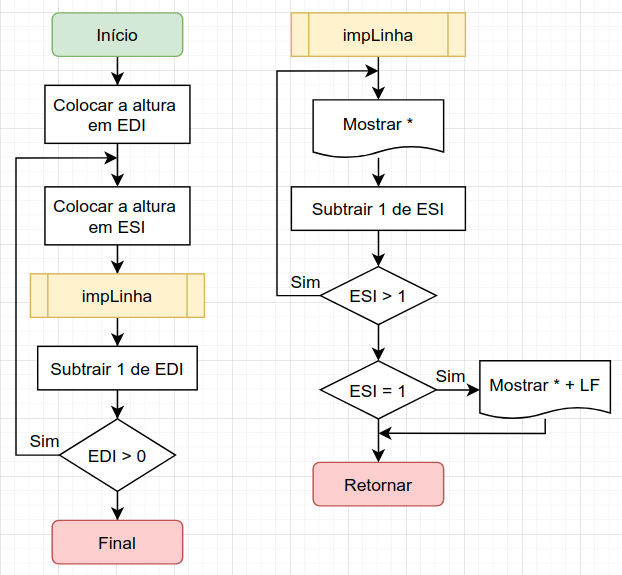
\includegraphics[width=0.6\textwidth]{Pictures/cap03/programa31}
	\caption{Fluxograma do Programa \textbf{Quadrado}}
\end{figure}

Criar um arquivo chamado "quadrado.asm" e começamos com a seguinte codificação:
\begin{lstlisting}[]
%include 'bibliotecaE.inc'

SECTION .bss
  lado resb 0x1 ; Valor do Lado Inicial

SECTION .text

global _start

_start:
  mov byte[lado], 0x4  ; Valor inicial do Lado
  mov edi, dword[lado]
\end{lstlisting}

Apenas para facilitar nossa definição do tamanho do quadrado criamos um marcador chamado 'lado', então definimos seu inicial para 4 (ou seja teremos um quadrado de 4 por 4, mude-o a vontade para testar outros tamanhos). Colocamos o valor de lado em \textbf{EDI} (que controla a quantidade de linhas), para o marcador \textbf{inicio}.

O interessante aqui é observamos como são realizadas as operações de movimentação entre um valor para um marcador da seção .bss e deste para um registrador. Do lado .bss usamos seu tipo que no caso é \textbf{byte}, porém quando vamos enviar para o registrador utilizamos \textbf{word}. 

Montamos o corpo principal:
\begin{lstlisting}[]
inicio:
  mov esi, dword[lado]
  call impLinha
  sub edi, 0x1
  cmp edi, 0x0
  je saida
  jmp inicio	
\end{lstlisting}

A cada linha, o valor de lado deve ser colocado em \textbf{ESI} (que controla a quantidade de colunas, já que um quadrado tem a mesma quantidade de linhas e colunas), saltamos para o marcador de modo a mostrar uma linha. Reduzimos a quantidade de \textbf{EDI} e comparamos seu valor com 0, se for igual saltamos para o marcador \textbf{saida} caso contrário retornamos para o \textbf{início}. Ou seja, este será o bloco principal do programa que gera todas as linhas do nosso quadrado.
\begin{lstlisting}[]
impLinha:
  mov edx, 0x1
  call impEstrela
  sub esi, 0x1
  cmp esi, 0x1
  jg impLinha
  mov edx, 0x2
  call impEstrela
  ret
\end{lstlisting}

No marcador \textbf{impLinha} usamos o valor de EDX em 1 para mostramos um '*' na saída do terminal, reduzimos o valor de \textbf{ESI} e se este for maior que 1 retornamos para o marcador \textbf{impLinha}. Quando o valor de \textbf{ESI} não for maior que 1, usamos o valor de EDX em 2 para mostramos "* + LF" (para saltar de linha) e retornamos para o ponto que nos chamou.
\begin{lstlisting}[]
saida:
  mov eax, SYS_EXIT
  mov ebx, EXIT_SUCESS
  int SYS_CALL	
\end{lstlisting}

Neste ponto apenas fazemos as movimentações para terminar o programa. Mas calma que ainda existem mais dois marcadores importantes no conjunto. Podemos agora imprimir quadrados de vários tamanhos, bastando apenas alterar os valores iniciais de \textbf{EDI} e \textbf{ESI}.

\section{Programa 3.2 - Pirâmide}\index{Quebrar a Cabeça}
Criar uma pirâmide de Asteriscos com base no valor da altura, por exemplo, se essa for 3 a pirâmide deve ser mostrada da seguinte forma:
\begin{lstlisting}[]
  *
 ***
*****
\end{lstlisting}

Para um valor 4, sairá assim:
\begin{lstlisting}[]
   *
  ***
 *****
*******
\end{lstlisting}

O que mais gosto desse desafio é que apresenta um elemento que não estamos vendo, os espaços iniciais, temos aqui duas perguntas que devemos resolver:
\begin{enumerate}[nolistsep]
	\item Quantidade de espaços em cada linha.
	\item Quantidade de * adicionados a partir da 2ª linha.
\end{enumerate}

Pensemos assim, se a altura passada for 5, na primeira linha quantos espaços em branco iniciais temos? Isso mesmo 4, mas essa é a resposta errada, na verdade temos a altura menos 1 (já que estamos na 1ª linha), na segunda linha a resposta não muda, é a altura menos 2 (agora estamos na 2ª linha). Agora vamos focar na segunda pergunta, temos 1 na 1ª linha, e são adicionados mais 2 asteriscos a cada linha.

\begin{figure}[H]
	\centering
	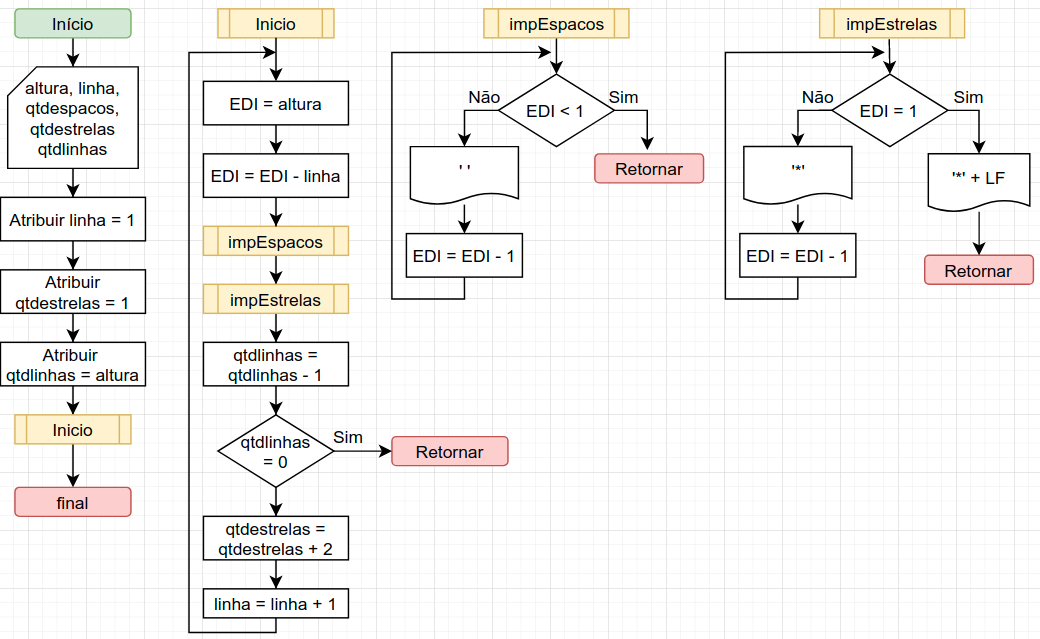
\includegraphics[width=0.75\textwidth]{Pictures/cap03/programa32}
	\caption{Fluxograma do Programa \textbf{Pirâmide}}
\end{figure}

Criar um arquivo chamado "piramide.asm" e começamos com a seguinte codificação:
\begin{lstlisting}[]
%include 'bibliotecaE.inc'

SECTION .bss
  altura      resb 0x4 ; Altura (fixa)
  linha       resb 0x4 ; linha atual
  qtdespacos  resb 0x4 ; Qtd de espacos
  qtdestrelas resb 0x4 ; Qtd de estrelas
  qtdlinhas   resb 0x4 ; Qtd linhas ja impressa

SECTION .text

global _start
\end{lstlisting}

Essa é a parte fácil: Codificar. Trata apenas de uma simples tradução para o nosso fluxograma que já escrevemos. Gostaria muito que as pessoas observassem que NUNCA podemos iniciar a codificação se primeiro não temos as respostas para nosso problema, seria uma simples perda de tempo (ou se prefere tentativa e erro).E falando sério, é por isso que existem tantas piadas a respeito de programas errados ou de programadores fazendo besteiras pois tentam encurtar o caminho.

Seguimos agora para o início do marcador \textbf{\_start} no qual atribuímos os valores as nossas variáveis:
\begin{lstlisting}[]
_start:
  mov byte[altura], 0x8
  mov byte[qtdlinhas], 0x8
  mov byte[linha], 0x1
  mov byte[qtdestrelas], 0x1
\end{lstlisting}

Inicializamos os valores das nossas "constantes" que vamos utilizar como iniciais, apenas para facilitar. No marcador \textbf{inicio} é que realmente temos o coração do nosso programa:
\begin{lstlisting}[]
inicio:
  mov edi, dword[altura]
  sub edi, dword[linha]
  call impEspacos
  mov edi, dword[qtdestrelas]
  call impEstrelas
  sub byte[qtdlinhas], 0x1
  cmp byte[qtdlinhas], 0x0
  je saida
  add byte[qtdestrelas], 0x2
  add byte[linha], 0x1
  jmp inicio	
\end{lstlisting}

Movemos para \textbf{EDI} o valor da altura e subtraímos da linha atual (resposta da 1ª pergunta) e mostramos os espaços. Movemos para \textbf{EDI} o valor da quantidade de estrelas e mostramos os asteriscos. Reduzimos um na quantidade de linhas e verificamos se chegou a 0 para terminamos, caso contrário, adicionamos mais dois asteriscos na quantidade e mais um a linha atual e saltamos para o início do marcador.

\begin{lstlisting}[]
impEspacos:
  cmp edi, 0x1
  jl finalImpEspaco
  call impEspaco
  sub edi, 0x1
  jmp impEspacos
  
finalImpEspaco:
  ret  	
\end{lstlisting}

Para mostrar os espaços basta verificarmos o registrador \textbf{EDI} que contém a quantidade que deve ser mostrado, para isso logo no início já o comparamos com um e se for menor chamamos o marcador \textbf{finalImpEspaco} que retorna para quem nos chamou (isso é feito pois reparemos que na última linha não existe nenhum espaço). Saltamos para o marcador que vai mostrar um único espaço, reduzimos um na quantidade de \textbf{EDI} e retornamos para o início desse marcador.

\begin{lstlisting}[]
impEstrelas:
  cmp edi, 0x1
  je finalImpEstrela
  mov edx, 0x1
  call impEstrela
  sub edi, 0x1
  jmp impEstrelas

finalImpEstrela:
  mov edx, 0x2
  call impEstrela
  ret  	
\end{lstlisting}

Mais um marcador de controle, agora para a impressão dos asteriscos, basicamente a mesma coisa do anterior porém com a diferença que ao término devemos imprimir o asterisco que conterá o salto de linha. De resto temos uma repetição padrão do anterior.

\begin{lstlisting}[]
saida:
  mov eax, SYS_EXIT
  mov ebx, EXIT_SUCESS
  int SYS_CALL	
\end{lstlisting}

E finalmente a saída do programa e encerramento das chamadas. E estamos prontos para mostrarmos uma pirâmide de qualquer tamanho possível, recomendo que tente estender este programa para mostrar um "Losango" (basta continuar a impressão e inverter a pirâmide). 

\section{Programa 3.3 - Xadrez}\index{Quebrar a Cabeça}
Realmente desenhar um tabuleiro de Xadrez é um desafio para muitos programadores, pois existe uma intercalação entre '*' e ' ' principalmente nas linhas pois o que começava com '*' agora vai começar com um ' '. O resultado é bem bonito:
\begin{lstlisting}[]
* * * * * * * *
 * * * * * * * * 
* * * * * * * *
 * * * * * * * * 
* * * * * * * *
 * * * * * * * * 
* * * * * * * *
 * * * * * * * * 
\end{lstlisting}

Vamos começar com a criação de um arquivo chamado 'xadrez.asm' com a seguinte codificação:
\begin{lstlisting}[]
SECTION .text

global _start

_start:
  mov edi, 0x0
\end{lstlisting}

Criar esse efeito do Xadrez é interessante pois devemos controlar simultaneamente 2 laços usaremos para o primeiro o registrador \textbf{EDI} que controlará a quantidade de linhas. Seguimos para o bloco principal:
\begin{lstlisting}[]
montaTabuleiro:
  add edi, 0x1
  cmp edi, 0x9
  je saida
  mov esi, 0x0
  mov edx, 0x0
  mov eax, edi
  mov ebx, 0x2
  div ebx
  cmp edx, 0x0
  jg linhaIniciaEstrela 
  jmp linhaIniciaEspaco	
\end{lstlisting}

Todo o programa se concentra neste bloco. Adicionamos 1 ao controlador de linha (\textbf{EDI}) e verificamos se estamos na nona linha, se for o caso vamos para o marcador \textit{saida}. Movemos 0 para o controlador de coluna (\textbf{ESI}), agora vamos usar a técnica de saber se o número é par ou ímpar: movemos 0 para \textbf{EDX}, o valor do controlador de coluna para \textbf{EAX}, o valor 2 para \textbf{EBX}, realizamos a divisão em comparamos se \textbf{EDX} contém 0 (indicando número par) caso afirmativo saltamos para o marcador \textit{linhaIniciaEstrela} caso contrário incondicionalmente saltamos para o marcador \textit{linhaIniciaEspaco}.

\begin{lstlisting}[]
linhaIniciaEstrela:
  add esi, 0x1
  mov edx, 0x1
  call impEstrela 
  call impEspaco
  cmp esi, 0x7
  jl linhaIniciaEstrela
  mov edx, 0x2
  call impEstrela 
  jmp montaTabuleiro	
\end{lstlisting}

Neste bloco devemos imprimir uma linha começada com '*', para isso adicionamos 1 ao controlador de coluna, movemos 1 para \textbf{EDX} (de modo que não ocorra o salto de linha), mostramos um '*' e um ' ', verificamos se o controlador de coluna está em 7, caso seja menor retornamos ao começo do bloco. Caso contrário movemos 2 para \textbf{EDX} (indicando que agora queremos o salto de linha) e mostramos o '*' final e voltamos para o marcador \textbf{montaTabuleiro}.

\begin{lstlisting}[]
linhaIniciaEspaco:
  add esi, 0x1
  mov edx, 0x1
  call impEspaco
  call impEstrela 
  cmp esi, 0x8
  jl linhaIniciaEspaco
  mov edx, 0x2
  call impEspaco 
  jmp montaTabuleiro	
\end{lstlisting}

Neste bloco devemos imprimir uma linha começada com ' ', para isso adicionamos 1 ao controlador de coluna, movemos 1 para \textbf{EDX} (de modo que não ocorra o salto de linha), mostramos um ' ' e um '*', verificamos se o controlador de coluna está em 8 (pois precisamos de um '*' a mais), caso seja menor retornamos ao começo do bloco. Caso contrário movemos 2 para \textbf{EDX} (indicando que agora queremos o salto de linha) e mostramos o ' ' final e voltamos para o marcador \textbf{montaTabuleiro}.

\begin{lstlisting}[]
saida:
  mov eax, SYS_EXIT
  mov ebx, EXIT_SUCESS
  int SYS_CALL	
\end{lstlisting}

E finalizamos nosso programa e podemos imprimir nosso tabuleiro sem problemas.

% Final do Capítulo
\clearpage